\chapter{Einleitung}
\section{Hintergrund}
In diesem Dokument wird die Planung und Entwicklung des „Sonic Phone“ beschrieben. Das „Sonic Phone“ umfasst die Umsetzung einer nativen mobilen Applikation sowie den Einsatz von Technologien und die Erweiterung eines Ultraschallgeräts um zusätzliche Komponenten, um eine Datenübertragung zu einem mobilen Endgerät durchführen zu können. Durch die Befestigung des mobilen Endgeräts auf einer konstruierten Vorrichtung an der Ultraschallsonde können die übertragenen Bilder, mithilfe eines installierten Teilerspiegels auf der Oberfläche betrachtet werden. Durch die Überlagerung der Bildsequenz mit der Realität wird dem Betrachter die Möglichkeit gegeben, die Ultraschallbilder in situ zu betrachten und dadurch in das Objekt zu schauen.\\
Die Idee für dieses Projekt basiert auf einem Verfahren aus dem Jahr 2000 von G. Stetten et al., welches in der Wissenschaftlichen Veröffentlichung aus dem Jahr 2002 mit dem Titel „Towards A Clinically useful Sonic Flashlight“ vorgestellt wurde. Das Verfahren wurde als „Real Time Tomographic Reflection (RTTR)“ bezeichnet und umfasste die Entwicklung einer Apparatur, mit der Ultraschallbilder während einer Untersuchung in situ  betrachtet werden können. Die Apparatur wurde in mehreren Generationen weiterentwickelt und umfasste mehrere Prototypen, die mit unterschiedlichen Monitoren (liquid crystal display (LCD), field emission display (FED)) und mit unterschiedlichen Halterungen („pistol grip“, „pencil grip“) konstruiert wurden. \footcite{SonicFlashlight} 

\section{Motivation}
Bei der standardmäßigen Verwendung eines Ultraschallgerätes wird das aufgenommene Ultraschallbild auf einem Monitor dargestellt, das von dem Anwender betrachtet werden kann. Diese Trennung zwischen der Stelle, an dem das Ultraschallbild aufgenommen wird und der Betrachtung des Ultraschallbildes an einer anderen Stelle führt dazu, dass von dem Anwender immer zwischen der eigentlichen Interaktion mit seiner Hand und der Betrachtung des Bildes gewechselt werden muss. Das setzt eine sehr präzise Hand-Augen Koordination voraus, bspw. wenn ein medizinisches Instrument an der Ultraschallstelle eingeführt wird. Dieser Vorgang widerspricht der natürlichen Wahrnehmung bzw. führt zu einer Verzerrung der Realität. Dieser Umstand soll durch die Realisierung des „Sonic Phones“ behoben werden.
\section{Zielsetzung}
Ziel des Projekts „Sonic Phone“ ist die Entwicklung einer mobilen Applikation, die Erweiterung des Ultraschallgeräts und die Konstruktion einer Halterung für die Befestigung des mobilen Endgeräts und einem Teilerspiegel an der Ultraschallsonde (siehe Abbildung \ref{fig:sonic_phone_skizze}). Die entwickelte Software soll in der Lage sein, die Erfassung, Konvertierung und die Kodierung der Ultraschallbilder vorzunehmen (serverseitig). Während die Implementierung einer mobilen Applikation dafür verwendet wird, die übertragenen Daten zu dekodieren und das Ursprungsbild wiederherzustellen. Ein anschließender Verarbeitungsprozess schneidet die benötigten Informationen (Ultraschallbild, Bildinformationen, Farbskala) aus dem Ursprungsbild heraus und setzt ein neues Zielbild zusammen. Die zusammengesetzten Bilder werden anschließend kontinuierlich auf der Benutzeroberfläche angezeigt. Durch die Betrachtung des Zielobjekts durch einen Teilerspiegel und die Spiegelung der Benutzeroberfläche des mobilen Endgeräts kann der Anwender die Ultraschallbilder in situ betrachten. Um eine möglichst realitätsgetreue Übereinstimmung zwischen der Realität und dem aufgenommenen Ultraschallbild zu ermöglichen, müssen die eingesetzten Technologien, Komponenten und Methoden in der Lage sein, die Bilder in Echtzeit aufzunehmen, zu übertragen, zu verarbeiten und darzustellen.

\begin{figure}[h]
	\centering
	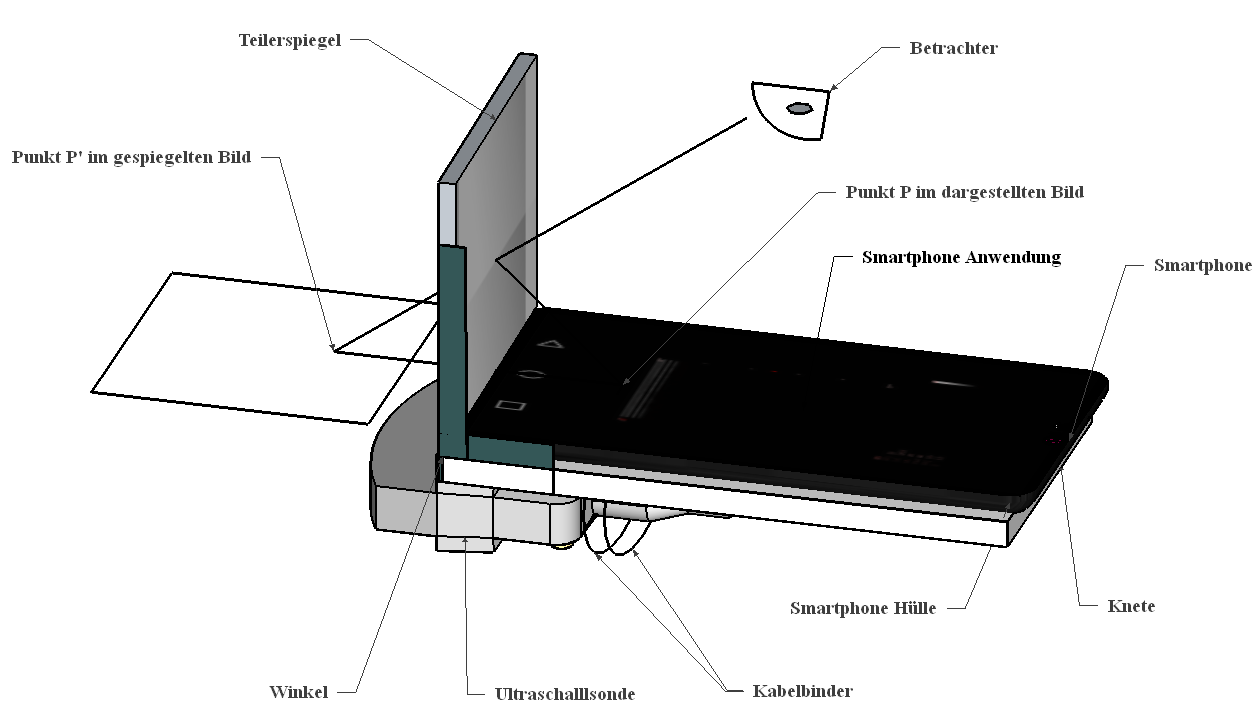
\includegraphics[width=1\textwidth]{Bilder/Einleitung/SonicPhoneSkizzeQuer.PNG}
	\caption{Sonic Phone Skizze}
	\label{fig:sonic_phone_skizze}
\end{figure}
